The following section of the report will describe the purpose of the Assembler Software component within YAMS, and provide in-depth details regarding its implementation and how this relates to YAMS as a whole.

\subsection{Introduction: Purpose of assembler}

The Assembler is the intermediate stage between the Parser and the Processor. The parser will have already taken the MIPS code provided to YAMS as input, checked its syntactic validity and transformed it into an internal representation that is simple to retrieve and manipulate.

Within the YAMS implementation we have closely modelled the real structure of a MIPS R3000 processor, thus internally the processor will retrieve instructions from its Memory Text Segment and execute them as in the real case. Therefore, logically the next phase in the process is to turn the internal representation of the parsed MIPS program into a binary representation that can be written to memory for the processor to execute.

The assembler carries out this task of assembly, while checking the semantics of the program as a whole e.g. checking whether the user refers to labels that aren't contained within the program, or whether all immediate values provided in decimal can safely be handled by the processor (i.e. no arithmetic overflow problems) once translated into their correct binary representation.


\subsection{XML Interaction}

As has already been mentioned within this document, XML has been extensively used within the project and is in fact at the core of the flexibility YAMS provides. All of the instructions supported by YAMS are stored within "Instruction\_file.xml," which is the Instruction Repository for the software. Intuitively, the Assembler needed to have a flexible design, handling instructions in a generic way such that it could cope with any new instructions that advanced users wished to implement.

Unlike both the Parser and the Processor, the Assembler would not have automatically generated handlers for each instruction it supports. Instead, it reads the required information from the XML at runtime and places this in tables which it can read and manipulate at will.


\subsection{Overview}


\subsubsection{COMPONENT DESIGN}

The following class diagram indicates the overall structural design of the Assembler, indicating which objects would maintain permanent links during YAMS runtime.


\begin{figure}
\begin{center}
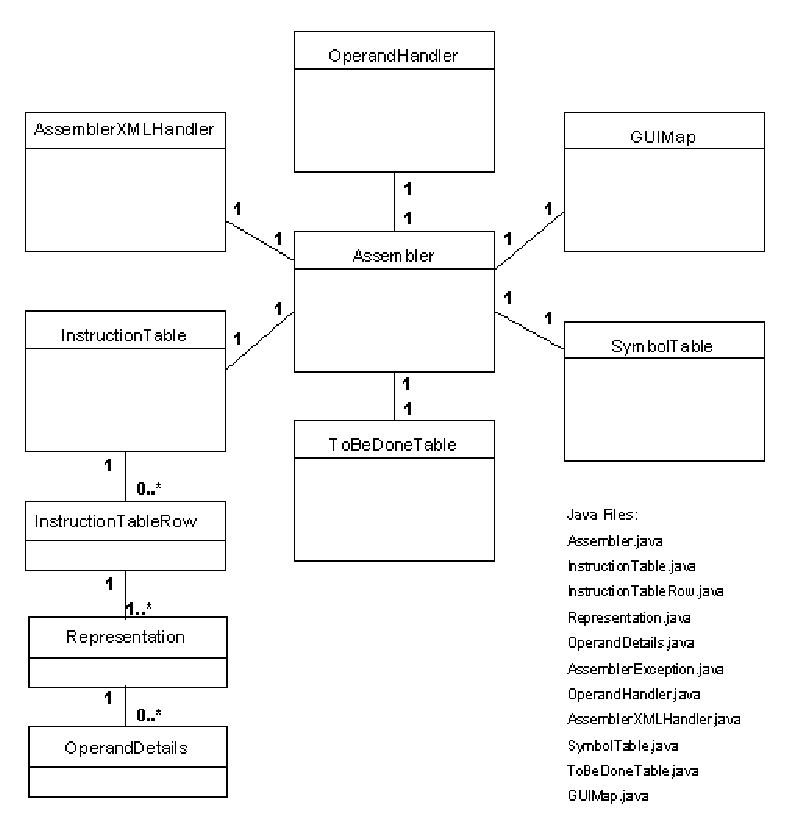
\includegraphics[width=8cm]{AssemblerDFD3.eps}
\caption{Class Diagram}
\end{center}
\end{figure}



\subsubsection{BRIEF COMPONENT DESCRIPTIONS}

As can be seen in the above diagram, there are a number of components within YAMS Assembler. They can be classified conceptually in two main areas. The assembler stores a lot of information (not just from the XML file, but also during assembly itself and for later stages within YAMS). Therefore there are isolated tables that simply store data and carry out operations limited to their data. The other components carry out the required tasks related to assembly utilising these tables accordingly. An overall summary of the components is outlined here, implementation details are provided later.

Tables used by the assembler:

\begin{description}
\item[InstructionTable]
The InstructionTable is designed to store the data read from the "Instruction\_file.xml" by the AssemblerXMLHandler in a predefined object structure which can be easily read by the Assembler.
\item[SymbolTable]
The SymbolTable is designed to store maps of symbols (e.g. a label within the Text segment OR a variable name in the Data segment) to their absolute addresses within memory.
\item[ToBeDoneTable]
The assembler will be reading and assembling the provided user code "line by line," therefore there will be occasions where an instruction cannot be immediately translated into machine code. For example, if we encounter a 'j \_location' (JUMP to \_location) MIPS instruction and \_location does not appear till some later line in the program, the assembler will not be able to work out the offset to assign the corresponding target jump instruction in binary. Therefore the translation of this instruction must be left till a later time, and the ToBeDone table contains a list of these instructions that need implementing along with the addresses to which they need assembling in memory.
\item[GUIMap]
The GUIMap component is a table whose existence is pertinent from the GUI point of view. It maps the line numbers of the original MIPS file to their assembled locations within memory, and can be used in the GUI to keep track of which line is being executed during a run of the program. 
\end{description}


Task handlers used by the assembler:

\begin{description}
\item[Assembler]
This is the core component of the overall Assembler structure, and it coordinates the activities of the other components. The public methods it provides will allow one entire program to be assembled into machine code, using the other components which it creates and maintains.
\item[OperandHandler]
This component is designed to take a provided set of operands for a given instruction, along with its core machine code representation (without any operand values filled in). It then performs the correct translation of the operands as required for the specific instruction and substitutes them into the machine code, leaving us with a machine word that can be written to memory ready for execution.
\item[AssemblerXMLHandler]
This component is designed to read from the "Instruction\_file.xml" instruction repository, by parsing through an internal representation of the file at runtime. It searches for expected tags and builds up a table of data on the instructions stored within the repository (table is InstructionTable described later).
\end{description}





\subsection{Assembler}

As can be seen in the class diagram already seen, the Assembler is the central object that coordinates the activities of the overall Assembly process. It therefore has control over the flow of all data, making critical decisions and calling other components in to carry out required tasks.

\subsubsection{External Interactions}
	Within the Assembler framework, the Assembler class is the only class with any external links to other YAMS components.
	\begin{description}
	\item[CREATION]
	An instance of the Assembler class is created by the YAMSConsole/YAMSGui objects (choice of console/Gui versions).

	\item[CALLED BY]
	The YAMSConsole/YAMSGui calls the public methods within Assembler class to assembler one MIPS Program (already Parsed to an AST).
	
	NOTE: The Assembler is designed to ONLY assemble ONE MIPS Program at a time, and has not been enabled with features that can cope with linking specific programs together. Therefore, the interface methods it provides allow only a single program to be submitted for assembly.

	\begin{verbatim}
	public void resetAssembler()
	public void assembleCode(LineList MIPSProgram)
	\end{verbatim}
	
	The resetAssembler() method resets the assembler ready to receive a new MIPS program, while the assembleCode method instructs the assembler to begin assembly on a new MIPS Program.
	
	\item[CALLS]
	The Assembler class maintains a reference to the Memory Manager within the Processor package to be able to write machine code words to memory directly as they are assembled.

	It also maintains a link to the StatisticsManager class (also within processor package) so that while it reads information from the XML file, it can build any tables that it needs to maintain statistics on individual instruction usage during program running etc.
	\end{description}
	
\subsubsection{Requirements}
	\begin{description}
	\item[INPUT]
	The assembler receives a LineList object (AST) from the Parser

	NOTE: The LineList object is described within the Parser documentation, but essentially provides a mapping from line-numbers to their contents:

	\begin{verbatim}
	Label                   _location:
	Instruction                         lw $a1,_x
	Label and Instruction   _start:     add $a1, $a2, $a3
	\end{verbatim}

	The contents of the Labels and the Instructions (including the values of the operands) are accessible through a variety of methods within this AST.

	\item[ASSEMBLY]
	Work through the LineList object "line-by-line," translate to machine code, encoding each instruction and associated operands into their machine code representation(s).

	\item[OUTPUT]
	32 Bit Words written to memory (Memory Manager) correctly representing the MIPS source code in binary (both TEXT and DATA segments), ready for the processor to begin its operation.	
	\end{description}
	
\subsubsection{Operation}
	There is one pre-operation phase that must be completed when YAMS is first created:

	\begin{enumerate}
	\setcounter{enumi}{-1}
	\item Assembler Instantiation
	\end{enumerate}
	
	There are three main stages of data flow for the Assembler class:
	
	\begin{enumerate}
	\item Table Initialisation
	\item 1st Pass Assembly
	\item 2nd Pass Assembly
	\end{enumerate}
	
	The implementation of these stages is outlined below:


	\begin{enumerate}
	\setcounter{enumi}{-1}
	
	\item ASSEMBLER INITIALISATION
	
		When an instance of YAMS is first created, the YAMSConsole or the YAMSGui classes (choice depending on required mode: console/gui) will create the core components of the software: Parser / Assembler / Processor. Therefore there are a number of stages the Assembler class must go through before any programs can be supplied for assembly.
	
		
		\begin{enumerate}
		
		\item Table Creation
	
		Must create tables it will need during assembly:
		
		\begin{itemize}
		\item InstructionTable
		\item SymbolTable
		\item ToBeDoneTable
		\item GUIMap
		\end{itemize}
	
		\item Operand Handler Creation
		\item Set internal MemoryManager reference
		
		The Assembler creation call will also contain an external reference to an already existing MemoryManager. Since the writeToLocation() method contained within this class will be used frequently throughout various stages of the Assembler, it is important to set a global reference to this object. 
	
		\item XML File Reading
	
		It is necessary to fill the InstructionTable with information on each of the instructions within the \verb"Instruction_file.xml" repository, since this will give us our supported instruction set. It would be possible to do this every time we reset the assembler, and capture any changes to the XML file (say if an instruction is added). However any changes to the instruction set require recompilation of YAMS to autogenerate the Parser and Processor handlers, so it is only necessary to read the XML once and copy the data to our tables.
	
		This is achieved by utilising the LoadTableFromXML(�) method within the AssemblerXMLHandler, which when provided with the XML File Path and the empty instruction table (just created in phase I), will fill the table. 
	
		\end{enumerate}
		
	\item TABLE INITIALISATION
	
		The Assembler must initialise all of the tables that it will require during its later phases. References to these tables will already exist within the Assembler class (see the previous section), they must now be reset (to clear the assembler of any old information on other programs), and the assembler be made ready to receive a new file. The following tasks are required:
	
		\begin{enumerate}
		
		\item Reset Tables
	
		SymbolTable	Reset any mappings from symbols to addresses.
		ToBeDoneTable	Reset any previous instructions that needed to be dealt with in the second phase.
		GUIMap	Reset any mappings from lines to addresses.
		
		\item Reset TEXT Address value
	
		During assembly, the global variable \verb"NEXT_TEXT_ADDRESS" will be used as the next free address in the TEXT segment where assembled instructions can be written to. Therefore, we must reset this when we are about to encounter a new program. Just like SPIM, and as set out in various definitions of the MIPS architecture, we define the TEXT segment to start at address 0x400000, and thus this is the required reset value.
	
		\item Reset DATA Address value
	
		A similar point to above, we must reset the \verb"NEXT_DATA_ADDRESS" to address 0x10000000, so that we effectively empty the DATA segment (from assembler's perspective).
	
		\item Reset Fixed Block Address Offset 
	
		YAMS can support fixed block addressing for certain instructions, for example lw. Please see the later OperandHandler section for further information on possible addressing modes. However, just in case this value has been changed at all during previous assemblies, we reset the value to 0x10008000.
	
		\end{enumerate}
		
	\item FIRST PASS ASSEMBLY
	
		Purpose?
	
		The assembler must now iterate through the LineList (AST) object that has been passed from the Parser and attempt to assemble the program.
	
		The following data-flow diagram will explain this process in further detail:
	
		The following are considered global variables for this data flow:
	
			\verb"NEXT_TEXT_ADDRESS",
			\verb"NEXT_DATA_ADDRESS",
			
		Data/Text Segment	(position of Assembler through file TEXT/DATA segment) 
	
		And for simplicity we are omitting graphically the GUIMap and Symbol Tables.
	
		\begin{figure}
		\begin{center}
		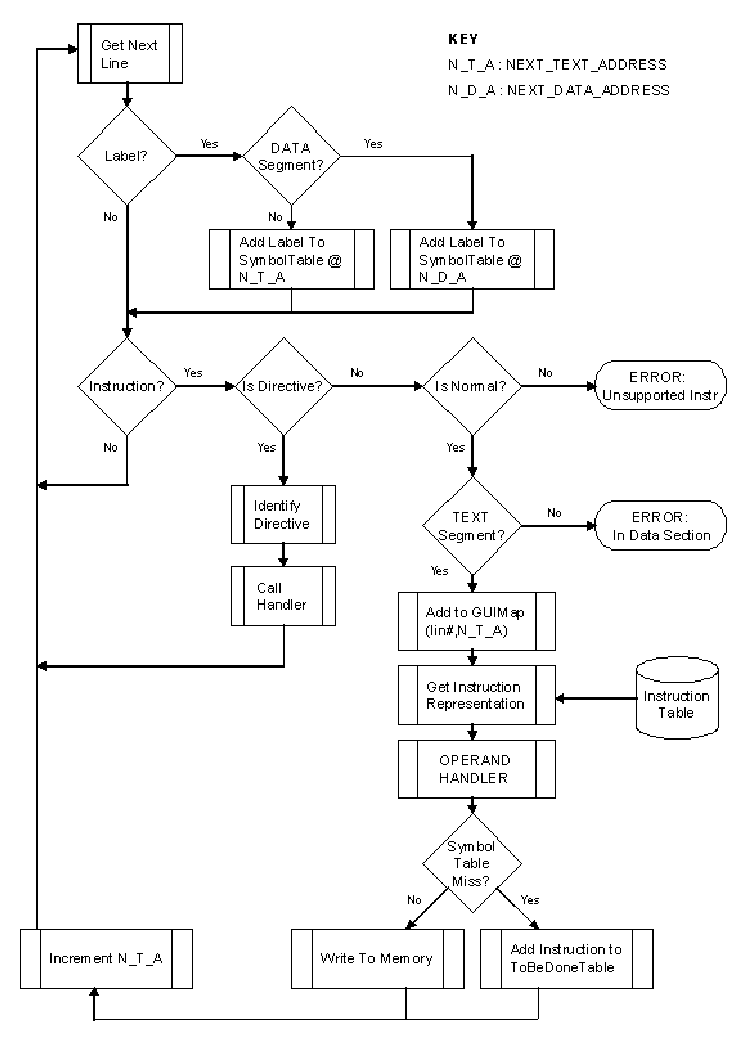
\includegraphics[width=8cm]{AssemblerDFD1.eps}
		\caption{DFD For 1st Pass}
		\end{center}
		\end{figure}
	
		When the Assembler encounters a new line it must first check if it contains a label or not e.g. \verb"_start:" If it does contain a label, then an entry needs to be added to the SymbolTable such that instructions can make references to the location and the assembler is able to resolve these addresses. If we are in the data segment then we add the label with the \verb"NEXT_DATA_ADDRESS", if the text segment then we add it with \verb"NEXT_TEXT_ADDRESS". Clearly, if we receive a label in the data segment then we MUST expect some variable definition as the next instruction, and this should have been already checked syntactically by the parser so no double-checks are performed here. Labels are allowed to be on their own lines within the TEXT segment, so there are no conflict problems there.
	
		The Assembler next checks whether the line contains an Instruction (which can be an Assembler Directive or a Normal Instruction). Logically, if we are dealing with an Instruction, the Directive/Normal check is carried out subsequently.
	
		If we encounter a directive (identified as a normal instruction with a "." prefix, we identify the type of directive (hard-coded into specific handlers) and excecute the code. Supported directives are as follows:
	
		\begin{description}
		\item .asciiz
		Writes a subsequently defined string to the DATA segment in memory using Ascii encoding.
		\item .space
		Sets aside a specified number of bytes within the DATA segment, achieved by incrementing \verb"NEXT_DATA_ADDRESS" accordingly.
		\item .data
		Indicates the beginning of the data segment, changes global state variable in assembler (knows to expect variable definitions).	
		\item .text
		Indicates the beginning of the text segment, assembler will expect instructions).
		\item .word
		Encodes the specified word into binary and places it in the DATA segment.
		\end{description}
		
		Other MIPS directives currently have their handlers constructed within the source code, but are NOT implemented. This can be left as an extension to the project, to completed at a later date.
	
		NOTE: XML Problems: It was considered that the Directives be added to the XML file, instead of being hard-coded within the Assembler class. However, the sheer volume of code required for each handler implied that a fixed directive set should be kept. However, it would be perfectly possible to implement similar XSLT transformations to those used on the Parser / Processor to autogenerate these handlers if it were really necessary and this can be left as an Extension to YAMS.
	
		If we encounter a normal instruction that is in the TEXT segment (instructions in DATA segment are NOT allowed), then we add a mapping of the current line to the \verb"NEXT_TEXT_ADDRESS" to the GUIMap. Next we retrieve a Representation object for this current instruction name and operand types from the InstructionTable and pass these to the Operand Handler (described later) which attempts to correctly encode the operands and return the full machine code for the instruction. We now check if there has been an error in encoding operands in terms of a SymbolTable "miss." 
	
		These occur where we attempt to resolve an address of a symbol we have not yet encountered in the program (could occur later, for example a jump instruction to a later address). If we do have a "miss" then we must add the current instruction to the ToBeDoneTable (along with the start TEXT address where it should be written to) so we can attempt to encode it later, once we have passed through all of the label references in the program. We DO NOT write ANY of the machine code for this instruction to memory. If we have no symbol table problems then we go ahead and write all of the code for this instruction to memory. In both cases however, we increment the \verb"NEXT_TEXT_ADDRESS" variable so that space is left for when the second pass takes place.
		
		The Assembler then moves back to the next line in the AST.
	
		
	\item SECOND PASS ASSEMBLY
	
		Purpose? Why is a second pass required?
	
		As has already been detailed, a second assembly pass is required at this stage, as there will be some instructions which had unresolvable addresses at that particular point in assembly. The second pass is NOT through the whole program again, but rather only on those instructions that were added to the ToBeDoneTable.
	
	
		During this phase the Assembler iterates through the Instructions stored in the ToBeDoneTable. It then handles the instructions in a very similar way to that already described within the previous 1st pass section. It retrieves the Representation and invokes the OperandHandler. This time however, if we get a SymbolTable "miss" then we must throw an error. By this point, our symbol table should contain all of the label->address mappings for the entire MIPS program. Therefore if the label is not in the SymbolTable, then it cannot be in the program and we must indicate to the user that semantically speaking this program is erroneous. This semantic check is something that the parser cannot identify and is vital to the checking validity of a program.
	
	\end{enumerate}






\subsection{OperandHandler}

\subsubsection{XML}
	One point that must be again highlighted regarding the structure and operation of the OperandHandler refers to the requirement for flexibility within YAMS. Since all the instructions are found in this repository and there is no hard-coding of instructions, then the OperandHanlder must be constructed to deal in the most generic way with the data it retrieves from the \verb"Instruction_file.xml."

\subsubsection{Requirements}
	
		\begin{description}
		\item[INPUT] Receives a combination of operands:
	
		\verb"String machineWord" A single 32 bit bitstring, which is an "uncoded" machine code representation of some of the instruction which is required to be translated.
		\verb"int address" An integer representing the current text address (\verb"NEXT_TEXT_ADDRESS" from Assembler).
		\verb"List opList" A list structure containing the Operand objects retrieved from the current Instruction representation (passed from parser).
		\verb"String opsCoding" A coded representation of the types of the operands in the list above.
		\verb"int line" The current line number of the Instruction
		\verb"Instruction current" The full instruction itself from the original LineList AST.
	
		The final two operands imply redundant reference to certain objects, but note that they are used to highlight any errors encountered with the whole line.
	
		NOTE: "uncoded" refers to machine code that hasn't had the correct values for its operands substituted yet e.g. 001000bbbbbaaaaacccccccccccccccc
	
		NOTE: Some instructions within the supported set can be multiple words in length, and the Assembler essentially will pass the OperandHandler a SINGLE word from this representation, and the operands themselves ready to be substituted. The other variables are used to setup the handler to translate these operands correctly pre-substitution e.g. if one operand is a label, then the OperandHandler must establish whether the offset should be calculated from the current address or from the \verb"FIXED_LINE_ADDRESS" (see addressing modes section later in this report).
		
		\item[HANDLING] The handler must encode the provided operands, and substitute their translated values into the provided "uncoded" machine word. 
	
		\item[OUTPUT] Returns a machine word which is fully coded, with all operands successfully substituted into their correct positions, ready to be written to memory. Must also provide an indication of whether there has been some error in referencing the SymbolTable (referencing label not yet encountered in the MIPS program).
		\end{description}
	
\subsubsection{Operation}

		The OperandHandler has been created (by the Assembler class) with references to:

		SymbolTable,
		ToBeDoneTable,
		InstructionTable

		As explained in the Requirements section above, it must now attempt to encode a SINGLE machine word using the provided operands.

		Diagrams

		The following data flow diagram shows the main phases involved in encoding a single machine word using the OperandHandler when the encodeOperands() call is made from the Assembler.

		Global variable used throughout the diagram:

		List translatedList 	List of encoded operands, in machine code.

		\begin{figure}
		\begin{center}
		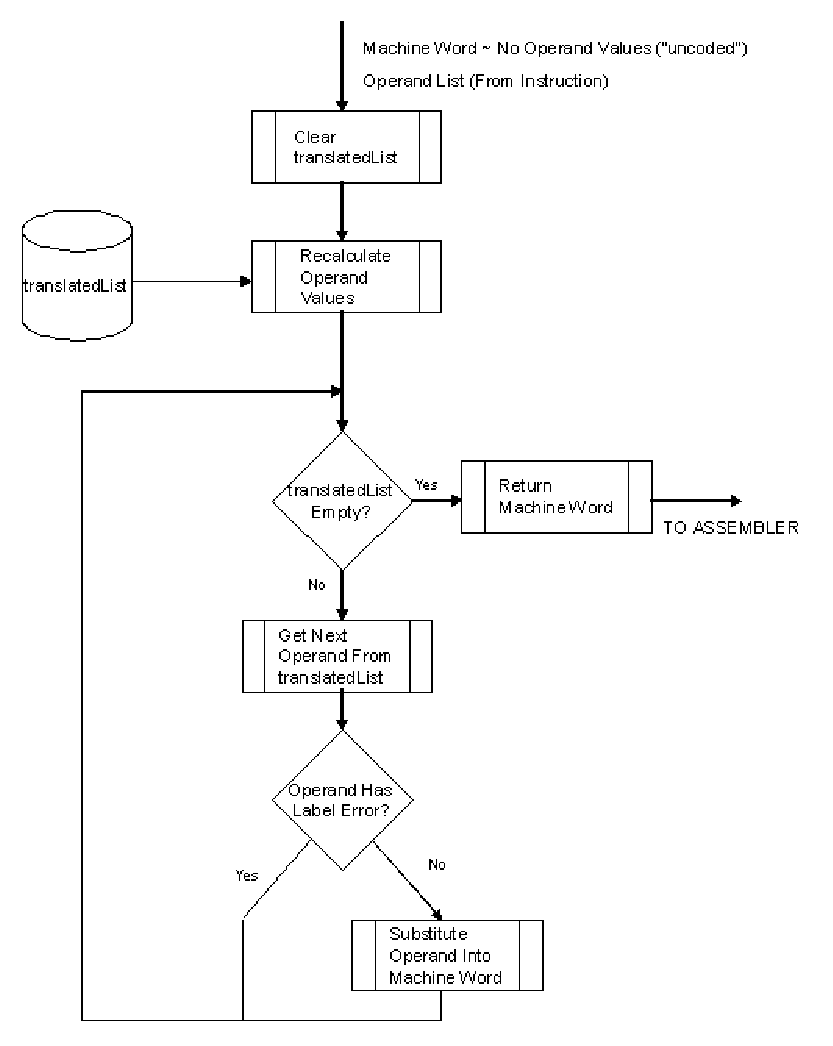
\includegraphics[width=8cm]{AssemblerDFD2.eps}
		\caption{DFD For OperandHandler encodeOperands() call}
		\end{center}
		\end{figure}

		Firstly, the handler must clear the translatedList, to flush out any previously encoded operand values. It then recalculates the values of the operands in the operandList provided to the OperandHandler, adding them to the translatedList (process described subsequently). With these newly calculated operands, we iterate through this list and replace their corresponding entries in the provided "uncoded" machine word in order. For example any substrings of "a" contained within the machine word are replaced by the FIRST entry in the translatedList. During this process if an operand has encountered a SymbolTable "miss" (referred to in Assembler-1st/2nd pass documentation) then its value is set to a recognised "ERROR" value. If this value is found, clearly this value isn't substituted into our output machine word. When the translatedList is exhausted, the substituted machine word is returned.

		Such exhaustive methods for replacing the operands must be employed since the structure of any instruction is not known to the OperandHandler due to the XML requirements. Thus, it must attempt to anticipate any combination / location of operands within each machine word.

		An example substitution:

\begin{verbatim}
addi rd, rs, imm	001000bbbbbaaaaacccccccccccccccc
                           rs    rd    immm

Operand Encoding
 $a1 = 00101
  20 = 0000000000010100

Substitution		00100000101001010000000000010100
\end{verbatim}


		The operands are recalculated for every word that is required to be encoded. Essentially, the list of provided operands is iterated through, and its type identified (e.g. Register, Immediate).

		The typing system for operands within the OperandHandler has to be necessarily more complex than those used within the Parser, since for certain operands the assembler must know more detailed information. The types supported are as follows:

\begin{table}
\begin{center}
	\begin{tabular}{|l|l|}
	\hline
	Character Code	&	Meaning \\
	\hline
	0	&	$<=$16 Bit Twos Complement Immediate \\
	a	&	32 Bit Twos Complement Immediate \\
	1	&	Register \\
	2	&	Label \\
	3	&	Address \\
	4	&	Add: Immediate \\
	5	&	Add: Immediate(Register) \\
	6	&	Add: Label \\
	7	&	Add: Label\_Plus\_Immediate \\
	8	&	Add: Label\_Plus\_Immediate\_Register \\
	c	&	Add: Label\_Minus\_Immediate\_Register \\
	9	&	Add: Register \\
	b	&	no operands \\
	\hline
	\end{tabular}
\caption{Operand Types}
\end{center}
\end{table}

		Therefore, the OperandHandler will identify a code for each of the Operands, and form an "OpCode" for this particular Operand Combination e.g. sub REGISTER REGISTER REGISTER has "OpCode" = 111. For each instruction stored in the XML there will be a unique machine code and associated operand information for each supported "OpCode." Therefore there will be different machine code representations for 111 than for 110 within the machine code, since it may be required that other instructions will be needed for the latter "OpCode" (say moving the immediate into a register before performaing the sub).

		Further details on the operands are stored within the instruction repository, including the accuracy with which to encode in binary and which bits to include in your final substitution. These details are retrieved from the InstructionTable and set the handler to a specific mode defined by a variety of variables. 

		The operand value provided with the MIPS instruction is then evaluated within the bounds of this mode, and added to the translatedList as described before. This method of setting the handler to a specific mode and then starting evaluation is necessary to provide the flexibility of being able to create a variety of instructions. 

		NOTE: For more information on the structure of the XML Representation of instructions please refer to the "Guide To Instruction Addition" within this documentation. This will also indicate the various addressing modes that are available to any instructions.


		




\subsection{AssemblerXMLHandler}

\subsubsection{Requirements}

	\begin{description}
	\item[INPUT]
	Provided with a file path to the \verb"Instruction_file" XML Instruction Repository and a reference to the empty InstructionTable. 
	\item[HANDLES]
	Must read the XML File, locate the \verb"<Instruction>" tags containing data on each instruction, and add this data to the InstructionTable
	\item[OUTPUT]
	Create an object based representation of the information stored in the file-based Instruction Repository.
	\end{description}
	
\subsubsection{Operation}

	The AssemblerXMLHandler achieves its objectives by using the already existing XML parsers included in the Java release. In this case, a DOM parser has been used.

	\begin{verbatim}
	DocumentBuilderFactory factory = DocumentBuilderFactory.newInstance();
	try {
	  DocumentBuilder builder = factory.newDocumentBuilder();
	  yams.util.FileReader fr = new yams.util.FileReader();
	  Document document = builder.parse(fr.readFile(xmlFilePath));
	  NodeList children = document.getChildNodes();
	}
	\end{verbatim}

	The DOM Parser automatically reads the XML file and generates an internal tree representation of the structured XML. This tree is then navigated through, and a series of hard-coded handlers attempt to match the values stored in these nodes to predefined tags, specified below.

	
\begin{verbatim}
<Instructions>

  <Instruction>
    <Name></Name>
    <OperandTypes></OperandTypes>
    <Javacode></Javacode>
    <Type fixedRt="true"></Type>
    <MachineCodeRepresentations>
      <Representation>
        <OperandsCoding></OperandsCoding>
        <MachineCode></MachineCode>
        <Operands>

        </Operands>
      </Representation>
    
    </MachineCodeRepresentations>
    <Help>
      <FullName></FullName>
      <Format></Format>
      <Description></Description>
    </Help>
  </Instruction>

<Instructions>
\end{verbatim}

	As soon as certain tags are encountered, the handler adds the required information to the InstructionTable. For example when the \verb"INSTRUCTION_TAG" is encountered, then a new InstructionTableRow is created and added to the InstructionTable to contain all the information regarding the new instruction. As the navigation continues deeper into the tree beneath the \verb"INSTRUCTION_TAG" further objects are created and then added appropriately to the correct entry in the InstructionTable.

	The following indicates the events that occur at each tag encounter:

\begin{verbatim}
\\ NAVIGATE THROUGH TO LOWER LEVEL
private static String INSTRUCTIONS_TAG = "Instructions";

\\create new InstructionTableRow
private static String INSTRUCTION_TAG = "Instruction";

\\subsequent information appears in InstructionTableRow
private static String INSTRUCTION_TYPE_TAG = "Type";
private static String CORE_TAG = "CoreMachineCode";
private static String NAME_TAG = "Name";

\\create new Representation
private static String REPRESENTATION_TAG = "Representation";

\\subsequent information appears in Representation
private static String OPERANDS_CODING_TAG = "OperandsCoding";
private static String MACHINE_CODE_TAG = "MachineCode";

\\ NAVIGATE THROUGH TO LOWER LEVEL
private static String OPERANDS_TAG = "Operands";

\\create new OperandDetails
private static String OPERAND_TAG = "Op";

\\subsequent information appears in OperandDetails
private static String OPERANDS_TYPE_TAG = "Type";
private static String OPERANDS_NUMBER_TAG = "Number";
private static String OPERANDS_ENCODE_BITS_TAG = "EncodeBits";
private static String OPERANDS_OUTPUT_BITS_TAG = "OutputBits";
private static String OPERANDS_MASK_TAG = "Mask";
private static String OPERANDS_OFFSET_MODE_TAG = "OffSetMode";
private static String OPERANDS_TAG = "Operands";
\end{verbatim}

	NOTE: A further implementation point to note is that the handler has also been used to build a StatisticsManager table for keeping count of how many times a particular instruction has been used within any given execution. Therefore every time the \verb"NAME_TAG" is encountered for an instruction, a method in the StatisticsManager is called to add this name to its table as a new entry.








\subsection{Tables}

The remaining components within the Assembler are simply table structures that are utilised by the Assembler, the OperandHandler and the AssemblerXMLHandler objects. Their definitions have already been discussed in the initial section of this chapter of the report, thus subsequent sections will only contain some specific implementation points:

Some general implementation points are common to all tables used within the assembler package:

Wherever possible, TreeMap structures have been used to store all mappings / required indexings. A TreeMap is a memory structure which stores (Key,Value) pairs where both are Objects. It is memory efficient, and very effective in terms of both in storage and retrieval times. The other advantage of using this structure is that almost all of the table accesses used within the assembler are random index accesses and do not need iteration across the whole structure. For example, queries to the InstructionTable consist of asking for a specific entry where the name = "queryString."

Another common feature across all the tables is the use of multiple \verb"get____()" and \verb"set____()" methods. For structures that have nested TreeMaps, there are \verb"add___()" methods to enable easy addition of objects to existing TreeMaps.

Finally, all the tables have reset features, allowing their contents to be wiped clean, while not deleting the object.

\subsubsection{INSTRUCTIONTABLE}

	\noindent \textbf{Structure}
	
	\begin{verbatim}
	TreeMap instructionMap
	  KEY = Instruction Name (String)
	  VALUE = Instruction Info (InstructionTableRow)
	\end{verbatim}
	
	\noindent \textbf{Description}
	
	The InstructionTable stores data from the \verb"Instruction_file" on each instruction to be supported by the assembler. In actuality, the InstructionTable uses a TreeMap to store objects of the type InstructionTableRow, which contains more information on the instruction and further links to other objects containing other details.
	
	Hierarchically, when considering all levels of linking (please see Figure 1) the InstructionTable contains references to the following objects:
	
	\begin{itemize}
	\item InstructionTableRow
	\item Representation
	\item OperandDetails
	\end{itemize}
	
	The definitions of the structure of these objects is included within this section of the documentation.
	
	NOTE: The implementation of InstructionTable also contains a mapping in the reverse direction from machine code -> instruction name. This has been included within the assembler to enhance debugging of pseudo-instructions. It enables the assembler to automatically locate the name of any given sub-instruction within a more complex pseudo-instruction, and print it for the user to identify what exactly is being identified. This feature is not necessary for the general implementation, but has been left within the project since it is possible extra instructions may be added to YAMS at a later date.
	
	\begin{verbatim}
	INSTRUCTIONTABLEROW
	
	String intructionName
	String instructionType
	String coreMachineCode
	TreeMap representations	
	  KEY = Operand Code (String)
	  VALUE = Specific Representation (Representation) 
	
	REPRESENTATION
	
	String operandsEncoding
	String machineCode
	TreeMap representations	
	  KEY = Operand Number (Integer)
	  VALUE = Operand Details (OperandDetails) 
	
	OPERANDDETAILS
	
	int operandNumber
	String operandType
	\end{verbatim}
	
	
		
\subsubsection{GUIMAP}
			
	\textbf{Structure}
	
	\begin{verbatim}
	TreeMap table
	  KEY = Line Number (Integer)
	  VALUE = Absolute Memory Address (Integer)
	\end{verbatim}
	
	\noindent \textbf{Description}
	
	The GUIMap maps between line numbers from the LineList AST provided initially by the parser and their absolute memory addresses.
	
	
\subsubsection{SYMBOLTABLE}
	
	\noindent \textbf{Structure}
	
	\begin{verbatim}
	TreeMap table	
	  KEY = Symbol (String)
	  VALUE = Absolute Memory Address (Integer) 
	\end{verbatim}
	
	\noindent \textbf{Description}
	
	The SymbolTable maps between the symbol (e.g. \verb"_location") and its absolute memory address. 
	
	
	
\subsubsection{TOBEDONETABLE}
	
	\noindent \textbf{Structure}
	
	\begin{verbatim}
	TreeMap table	
	  KEY = Number (Integer)
	  VALUE = Currently Note Assembled Instruction (Instruction) 
	\end{verbatim}
			
	\noindent \textbf{Description}
	
	The ToBeDoneTable provides essentially a tree map of instructions that require re-assembling due to their containing a symbol which could not be found within the SymbolTable during the first assembly pass.

	

\subsection{Summary}

The structure of the assembler has been designed and implemented to cater for dealing with a dynamic instruction set. Unlike the Parser and the Processor, the Assembler doesn't have handlers that are rebuilt every time the instruction set changes. Instead, great flexibility has been provided in the OperandHandler and Assembler classes to allow all of the information regarding instructions to be read at run-time.
